\documentclass[11pt]{article}
\usepackage[margin=1in]{geometry}
\usepackage{amsmath,amssymb,amsthm}   % American Mathematical Society packages for typesetting math.
\usepackage{enumerate}                % Allows me to control numbering format for ordered lists.
\usepackage{tikz}                     % We may this later in the semester for drawing diagrams with LaTeX code.
\usepackage{enumitem}                 % Allows me to customize numbers styles in ordered lists.
\usepackage{clrscode4e}

\newtheorem{theorem}{Theorem}
\newtheorem{claim}{Claim}
\theoremstyle{definition}
\newtheorem{problem}{Problem}

\newcommand{\ZZ}{\mathbb{Z}}    % Integers
\newcommand{\NN}{\mathbb{N}}    % Natural Numbers
\newcommand{\QQ}{\mathbb{Q}}    % Rational numbers.

% Replace these with your own information.  Remember to use \today in the \date command.
\title{SpaceMath: Project Progress Report}
\author{Nick Satriano, Yang Hong, Jimmy Zhu, Per Astrom}
\date{\today}

\begin{document}
\maketitle
\begin{enumerate}
\item \textbf{Overview} \\
As technology has rapidly evolved, many aspects of everyday life have become deeply entrenched in modern computers. The internet has enabled near-instant communication and is the most effective tool for information distribution, becoming increasingly accessible with the mass production of smartphones and laptops. As a result, the education system has modernized, utilizing online resources to distribute course material, upload assignments, and turn in homework. Students have adapted to the modern online learning environment, often choosing to forgo handwritten work in exchange for the convenience of typing. Though education has improved in many regards through the use of technology, a new issue has arisen:  the lack of a fast, convenient method to insert mathematical notation in digital documents. The current standard is the language LaTex, which requires the user to type out precise formatting rules that are difficult to remember and tricky to write correctly. For example, to write the equation \[ \int_{a}^{b} x^2 \,dx \]
with LaTex, a person would have to type: \verb| \[ \int_{a}^{b} x^2 \,dx \]|

Neither the slashes, the brackets, nor the comma are intuitive to include (unless one has learned them by heart) as these are not part of the visible output, they are just formatting rules.

On the other end of the spectrum are graphical user interfaces with on-screen buttons (such as a smartphone calculator application), which are easy to use but far too slow and cumbersome for longer inputs. It would not be practical to write a textbook in this way, for instance. It also requires special buttons that cannot be found on a standard keyboard, and few GUIs have more than the most basic mathematical symbols.

Our goal with SpaceMath is to make the simplest system possible for typing mathematics which a computer can understand and format. As our client, Dr. Farmer, put it: “Don’t force the author to write what they don’t need to”.
Using SpaceMath to output the same equation as above, the user may simply type: \verb|integral from a to b x^2 dx|

The SpaceMath form is more accessible for the user and transmits the actual meaning of the equation without formatting “noise”.

If the user get proficient to SpaceMath and knows more about the keywords, (s)he can type \verb|int_a^b x^2 dx| instead. We may see that this form is similar to the Latex input, but much shorter and thus easier for the user to view. Therefore, we may see SpaceMath devoted to be more accessible and more efficient than LaTeX in simple math equations type-ups.

\item \textbf{Current Status of the Project} \\
We have had two team meetings with our client, Dr. Farmer, thus far. During our first progress report meeting, we worked with Dr. Farmer to define standards for some ambiguous use cases, more specifically how SpaceMath should interpret these input strings:
\begin{enumerate}
\item[1.] \verb|$1/2+3$|
\item[2.] \verb|$1/(2+3)(4+5)$|
\item[3.] \verb|$sinx$|
\item[4.] \verb|$sinh$|
\item[5.] \verb|$rootN(M)$|
\item[6.] \verb|$sqrtM$|
\item[7.] \verb|$iso$ or $isomorphic$|
\end{enumerate}

We concluded that in the first two cases, if there is a lack of space before and after the  “$+$” operator in “$2+3$”, or in the second case in between the two multiplied terms “$(2+3)(4+5)$”, then the entire term should be placed in the denominator. If there is a space, then the added or multiplied term will be represented outside of the fraction (becoming its own term).

In the third and fourth case, we concluded that “sinh” should be interpreted as hyperbolic sine, and as a result, “sinx” must not be interpreted as “sine of x”. Instead, users must include a space after typing “sin” or “sine” in order to properly input the trig function.

For cases 5 and 6, we concluded that users should be able to input roots using the form “rootN(M)”, where N is interpreted as the index of the root, and M is interpreted as the radicand. For handling square roots, like in case 6, we will allow users to input the form “sqrtM”, which will be interpreted as square root of M.

Lastly, we discussed how keyword operators should be handled. We decided that it would be less intuitive for users if spaces were interpreted as valid input in multiple character operators like “divided by”, and as a result we are limiting these operators to be simple, spaceless strings. As with case 7, we decided that users will be able to input strings like “iso” or “isomorphic”, which will allow multiple user input cases for non-standard operators, most of which are not found on common keyboards. Overall, these resolutions did not massively alter the build of our product. \\

\textbf{Simple Demo} \\
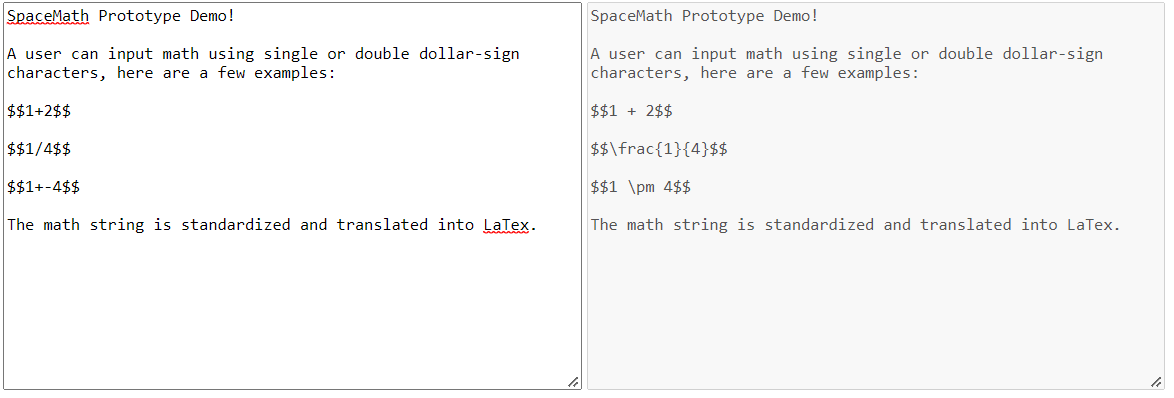
\includegraphics[scale=0.6]{image4.png} \\

\textbf{Testing the Output with MathJax} \\
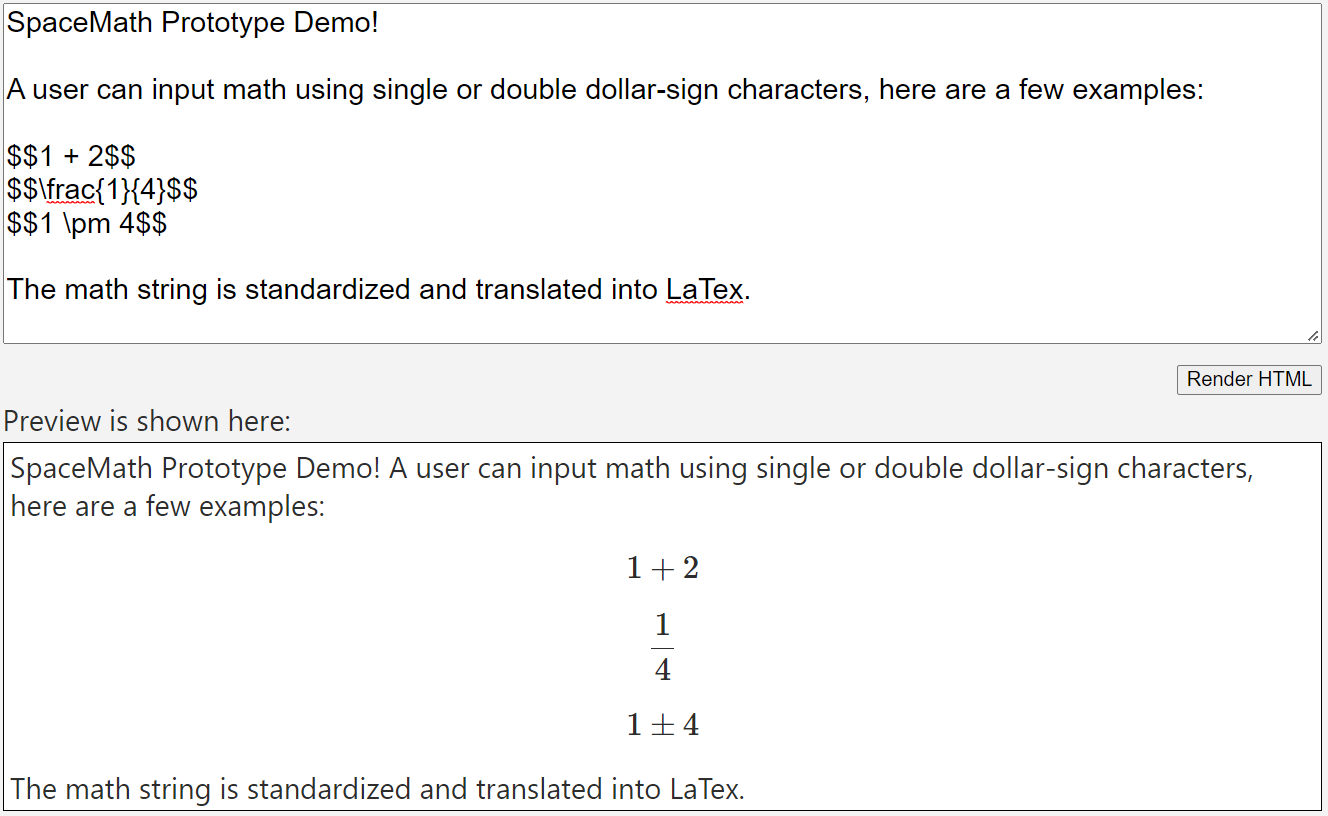
\includegraphics[scale=0.5]{image8.png}


\item \textbf{System Design} \\ 
In this section, we’ll introduce the process of how our program can translate SpaceMath texts into LaTex, together with the data structures and main algorithms used in the process. \\

\textbf{Programming Tools and Technologies} \\
We choose to implement SpaceMath in JavaScript, for the following reasons:
\begin{enumerate}
\item[1.] SpaceMath is aimed to be used in web applications and Javascript programs, being “the programming language of the web” can easily be inserted in HTML text with <script> tags and makes it straightforward to manipulate HTML elements, such as user-inputted text.
\item[2.] We considered TypeScript - a strictly typed version of JavaScript and a worthy alternative - however, JavaScript has less syntax (and thus a lower learning curve) and is more than sufficient for the scope of our project. With the simplicity of both our input data (nothing but strings) and stored data (maps containing mostly strings) there is little need for strict type checking.
\end{enumerate}
\textbf{Dictionary} \\
Before introducing the real algorithm, we first need to introduce the structure in which we store our data. We have a dictionary file which contains the information of keywords that are allowed in SpaceMath. 

There are many possible ways of representing mathematical symbols, we could construct objects internal to the code or store it as text in external files, such as in CSV format. We decided to use JSON-format, a lightweight and readable standard that uses simple map-format to store strings and numbers. It is more general and hence more flexible and adaptable to change and extension than creating specific class-objects. Whereas class-objects can only be used in functions that specifically support them, JSON data structures, being simple maps, can be used in all functions that . JSON is also very well-supported in JavaScript (being JavaScript Object Notation). An example of how we structure a mathematical symbol like: 
\begin{codebox}
\li "+": \{
\li \Do "alternative": ["plus"],
\li     "type": "operator",
\li     "priority": 10,
\li     "rule": \{"2,3": "\#1 + \#3"\}
    \End 
\li \}
\end{codebox}
\begin{itemize}
\item \textbf{“alternative”} is suggesting the other ways the user can type in this keyword. We will make use of it when we introduce translation in the future.
\item \textbf{“type”} is indicating which category the keyword lives in. We currently support types “operator” ($+$ $-$ \^ \_), “relation” ($>$ $=$ $<$), and “symbol” ($alpha$, $beta$, $pi$). Each category shares the same parsing rule.
\item \textbf{“priority”} is indicating the priority of the symbol when we are applying parsing. We mainly follow the PEMDAS (Parenthese, Exponentiation, Multiply, Divides, Add, Subtract) rule for priorities, and have appropriate priority for other symbols, assisting with consistent and correct translation.
\item \textbf{“rule”} stands for replacement rule and will be used in the combination process. It is a map in which the keys would be the possible tree node structures it can live in, and the corresponding value being the corresponding replacement rule for that situation. We will explain more details about it in the introduction of the combination process.
\end{itemize}
\textbf{BNF grammar to split text \& math} \\
The user input may contain pure text (not surrounded by the delimiters) and math text (surrounded by the delimiters). The algorithm first separates these parts, sends all math parts to the next step to convert them to LaTeX, then combines them back after the math parts are converted. \\

\textbf{Tree construction \& priority} \\
We choose the tree structure to be the form storing information when we parse the math input as it can keep the information and is easy to combine back to a string. The information each treenode contains other than its position, parent and children are its “value”, “key”, and “pair”.  “value” is a parsed piece of the original string, “key” tells which keyword is used under its parent, and “pair” indicates if it needs to be surrounded by a pair of parentheses.

We read the math string from left to right and construct the tree based on the keyword we find on the way. It would be complicated to introduce all the details in the process of parsing the string into a tree, so we will show the process by an example. \\

\textbf{Example:} \\
We’ll show how the math string $(3+4)/pi + 3$ goes through the process of tree parsing as an example. In the example, we will denote each tree node in the form $x(y)$, in which $x$ is the value and $y$ is the key of that tree node. 

When we scan the string from left to right, the first important thing we noticed is the left parenthesis "(". We then find the corresponding right parenthesis of it. In-between these parentheses is “$3+4$”. Therefore, we recursively call the tree construction function on “$3+4$”. 

Constructing a tree for “$3+4$” is not difficult - we can easily find the keyword “$+$” and recognize that it is an operation. The operation needs an argument before and after it, and our only choice is “$3$” and “$4$”. So the parse tree for “$3+4$” would be 
\begin{center}
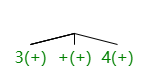
\includegraphics[scale=0.8]{image5.png} 
\end{center}
Now we put this tree into a holder variable and continue reading.the original string. After the right parenthese, the first keyword we find is “$/$”, which is an operator. It pulls out the tree structure in the holder as its left argument, and simply takes the rest of the string as its right argument. Hence the tree we have for this step is 
\begin{center}
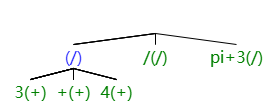
\includegraphics[scale=0.7]{image10.png} 
\end{center}
(Note for the left subtree, it has a property value of “pair” indicating it should be surrounded by parenthesis).

Our focus moves onto the rest of the string, which is $pi+3$. The first keyword here is the symbol $pi$. We just construct a simple tree for it: \begin{center}
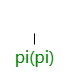
\includegraphics[scale=0.7]{image7.png}
\end{center}
and then place it into the holder variable.

The next keyword we met is “+”. As it is an operator, it takes the pi tree as the left argument and 3 as the right argument.
\begin{center}
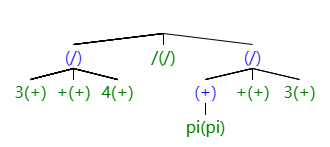
\includegraphics[scale=0.7]{image2.png}
\end{center}
Notice that “$pi+3$” in the tree has a key of “/”. Finding that the priority of ”$+$” is less than “/”, we notice that we need to adjust the order of the “+” siblings. We attempt to move to the parent, but that is already the child of the root. Thus we say the “+” should just live there, so we leave the left argument there, and move the “+” together with its right argument to the higher layer. After we made the adjustment, the tree would look like:
\begin{center}
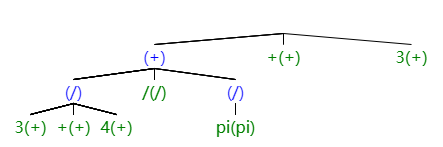
\includegraphics[scale=0.7]{image3.png}
\end{center}
And we have exhausted the string, so that would be how the final parse tree looks like. \\

\textbf{Tree Combination} \\
After we parsed the tree successfully, we’ll combine the tree back to a string. In this process, the replacement rules will work to make sure that the final string is a readable string in Latex that corresponds to the initial user input. Again, we use the previous example to show how tree combination works. Recall that the tree looks like 
\begin{center}
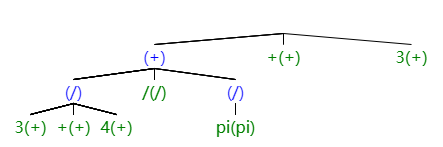
\includegraphics[scale=0.7]{image3.png}
\end{center}
For combination, we call the combine() function on the root node. Combine first call on all its children, then deal with the rest of the function, hence all leaves are operated the first.

We do nothing if the node is a leaf. Otherwise, we attempt to apply the rule. Let’s focus on the (/) on the left. All its children have the key “$+$”. The rule for “$+$” is \verb|{"2,3": "#1 + #3"}|. In English words, that means “If the keyword is the 2nd of 3 sibling, then replace the branch into "\verb|#1 + #3|", in which \verb|#i| means the content of the ith sibling”. Hence, the branch would be replaced by “$3+4$”. Recall that this branch has a parenthese property, so we need to have the parenthese there. (Interaction between operators \& parenthese will be added later). Hence the tree now looks like 
\begin{center}
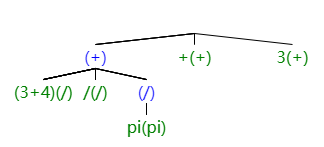
\includegraphics[scale=0.7]{image9.png}
\end{center}
The next thing we deal with is the other (/), in which the only child is pi. Its rule is \verb|{"1,1": "\\pi"}|, so it will be directly replaced by \verb|\pi|.The tree now looks like this: 
\begin{center}
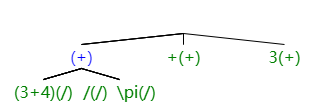
\includegraphics[scale=0.7]{image11.png}
\end{center}
Now, as all its children have finished the combine() function, we can work on the ($+$). The “/” works just like “$+$”, only with a different replacement rule: \verb|{"2,3": "\\frac{#1}{#3}"}|. Applying that, we have
\begin{center}
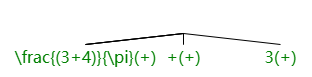
\includegraphics[scale=0.7]{image6.png}
\end{center}
The only thing left is the root and it is not hard to do that combination. Hence the final string we end up with is \verb|\frac{(3+4)}{\pi}+3|, which is the output we are looking for to input \verb|(3+4)/pi + 3|. \\

\item \textbf{Reflection on Challenges} \\
One major challenge we are having is to allow our program to be more expandable so our client can further add new keywords into the dictionary without changing any code. We decided to make the structure abstract and reduce the components of hard-coded processing. In other words, program to abstractions (not concretions). This means that we should only have hard-coded content for specific keywords (like parenthesis, the sup \& subscript, etc.). All other symbols should fall in some standard that can be covered by our dictionary structure.

Another challenge is that as the code expands, it becomes more difficult to reason about. making it hard to change and maintain. We may have to refactor the code at some point, to make it possible for Dr. Farmer to maintain the project in the future and make it easy to further extend. 

A difficulty with using scrum is that it takes time to use, and can feel like extra administrative work at times, getting in the way of the real work. But it is good practice for keeping track of things and making sure that progress goes in the right direction. \\

\item \textbf{Plan for the Rest of the Semester} \\
Here is a list of future works needs to be done:
\begin{itemize}
\item Interaction of parenthese with functions/operators (\verb|/, ^, _| etc may absorb the outermost pair of parentheses of its arguments)
\item implementation of functions
\item Implementation of multi-line sentence structure (cases, itemize, linear system)
\item Implementation of the translate Hashtable (so alternatives can be recognized in parsing), translation step (so all nodes are in standard form when combining)
\item Add in more keywords
\item Have specific rules for keywords which can be in multiple types: “$<$” for instance, it is a “relation” when surrounded by space, but the symbol “\verb|\langle|” if not. This may lives in M2Tree totally, or maybe we want to adjust the dictionary structure.
\item Add in the small space “\,” in Latex to indicate the existence of space multiplication
\end{itemize}
We plan to allow our program to support these functionalities listed above. After we have reached a stable demo, we may also apply a wider range of test cases in order to determine if we can refine/expand the depth of accepted input.

\end{enumerate}
\end{document}
